% Chapter 8

\chapter{Conclusions} % Main chapter title

\label{Chapter8} % For referencing the chapter elsewhere, use \ref{Chapter1} 

\lhead{Chapter 8. \emph{Conclusions}}

%----------------------------------------------------------------------------------------

In this dissertation, we provide two main contributions to the field of autonomous racing:

\begin{enumerate}
	\item We introduce a simple framework for comparing autonomous racing controllers using three key metrics: speed, safety and smoothness and accounting for statistical error using the P-Value method.
	\item With those metrics, we look at four key problems:
	\begin{itemize}
		\item How DQN performs compared to Wall Following (H1)
		\item How DQN using CNNs perform compared to NNs (H2)
		\item The ability of DQN to generalise to unseen tracks (H3)
		\item The ability of DQN to overcome the Sim2Real gap (H4)
	\end{itemize}
\end{enumerate}

We will first discuss those four hypotheses in Section \ref{reflexions}, then make some general conclusions in Section \ref{generalconclusions}, and finally propose possible future improvements to this project in Section \ref{futureworks}.

\section{Reflexions}
\label{reflexions}

\subsection{Hypothesis n°1}
\label{reflexions_h1}
When looking at the comparison between the lap time, average minimal LiDAR distance and average acceleration/deceleration metrics on the RedBull track (Figures \ref{h1_time}, \ref{h1_lidar}, \ref{h1_accel} and \ref{h1_decel}), we can draw 3 conclusions regarding Hypothesis n°1 (\textit{Deep Reinforcement Learning provides a real advantage, quantified by reliable metrics, for controlling an F1Tenth car over human control and PID-based methods like wall following.}):
\begin{itemize}
	\item  Regarding the speed metric (time to complete a full lap), Hypothesis n°1 appears to be verified for 2 DQN controllers: the CNN with reward functions n°2 and 3, with the latter performing the best. The hypothesis may also be verified for a NN with reward function n°2, but the experimental uncertainty is too high to confirm this result.
	\item Regarding the safety metric (average minimum LiDAR distance), Hypothesis n°1 appears to be verified for all DQN controllers apart from the NN with reward function n°1. The best performing controllers are the CNNs, with the reward function n°3 being the best.
	\item Regarding the smoothness metric (average acceleration/deceleration), Hypothesis n°1 is only verified by the CNN with reward function n°3 when looking at the average deceleration metric but is verified by all DQN controllers apart from CNN with reward function n°2 when looking at the average acceleration. 
\end{itemize}

Those conclusions were made by looking at the 95\% confidence intervals represented by the errors bars (in Figures \ref{h1_accel}, \ref{h1_decel}, \ref{h1_lidar}, \ref{h1_time}, \ref{h3_accel}, \ref{h3_decel}, \ref{h3_lidar}, \ref{h3_time}) as explained in  Chapter \ref{Chapter6}. \\
Hypothesis n°1 can then be checked using the P-Value method (more details are available in the Excel file at \url{https://github.com/HL-Boisvert/MSc_Project_HW}): \\

\begin{itemize}
	\item \textbf{Null Hypothesis (H0)}: CNNs provide no real advantage with reward functions 2 and 3 over Wall Following. 
	\item \textbf{Alternative hypothesis (H1)}: CNNs provide a real advantage with reward functions 2 and 3 over Wall Following.
\end{itemize}

Using the standard value of Alpha = 0.05 and an independent two-tailed T-test, we obtained the following results:

\begin{itemize}
	\item Time metric: comparing the 10-lap sample with reward function n°2 to the 10-lap sample with Wall Following gives $p-value=1,81 \cdot 10^{-12}<0,05$, which means the result is significant, and the Null Hypothesis can be rejected. With the reward function n°3, we get $p-value=7,29 \cdot 10^{-16}<0,05$: the result is also significant.
	\item Average acceleration metric: comparing the 10-lap sample with reward function n°2 to the 10-lap sample with Wall Following gives $p-value=1,14 \cdot 10^{-22}<0,05$, which means the result is significant, and the Null Hypothesis can be rejected. With the reward function n°3, we get $p-value=6,56 \cdot 10^{-10}<0,05$: the result is also significant.
	\item Average deceleration metric: comparing the 10-lap sample with reward function n°2 to the 10-lap sample with Wall Following gives $p-value=0,0094<0,05$, which means the result is significant, and the Null Hypothesis can be rejected. With the reward function n°3, we get $p-value=6,64 \cdot 10^{-23}<0,05$: the result is also significant.
	\item Average minimal LiDAR distance metric: comparing the 10-lap sample with reward function n°2 to the 10-lap sample with Wall Following gives $p-value=2,83 \cdot 10^{-18}<0,05$, which means the result is significant and the Null Hypothesis can be rejected. With the reward function n°3, we get $p-value=1,42 \cdot 10^{-22}<0,05$: the result is also significant.
\end{itemize} 

To conclude, the only DQN controller which verifies Hypothesis n°1 for the speed, safety, and smoothness metrics is the CNN with reward function n°3. This shows that a DQN controller has to be trained using a carefully chosen reward function to be efficient and that with the limited training time used in the experimental protocol, NNs don't verify the hypothesis. \\
However, it is likely that for a longer training time, the DQN would have been able to perform better, as the average reward during an evaluation epoch of several of the controllers was still increasing towards the end of the training, especially CNNs with reward functions 2 and 3 (Figure \ref{comparison_eval}). For those two controllers, the reward increased by over 30\% during the last 30 evaluation epochs, unlike the other controllers, which didn't show any significant reward increase over that time.

\begin{figure}
    \centering
    \begin{minipage}{0.45\textwidth}
        \centering
        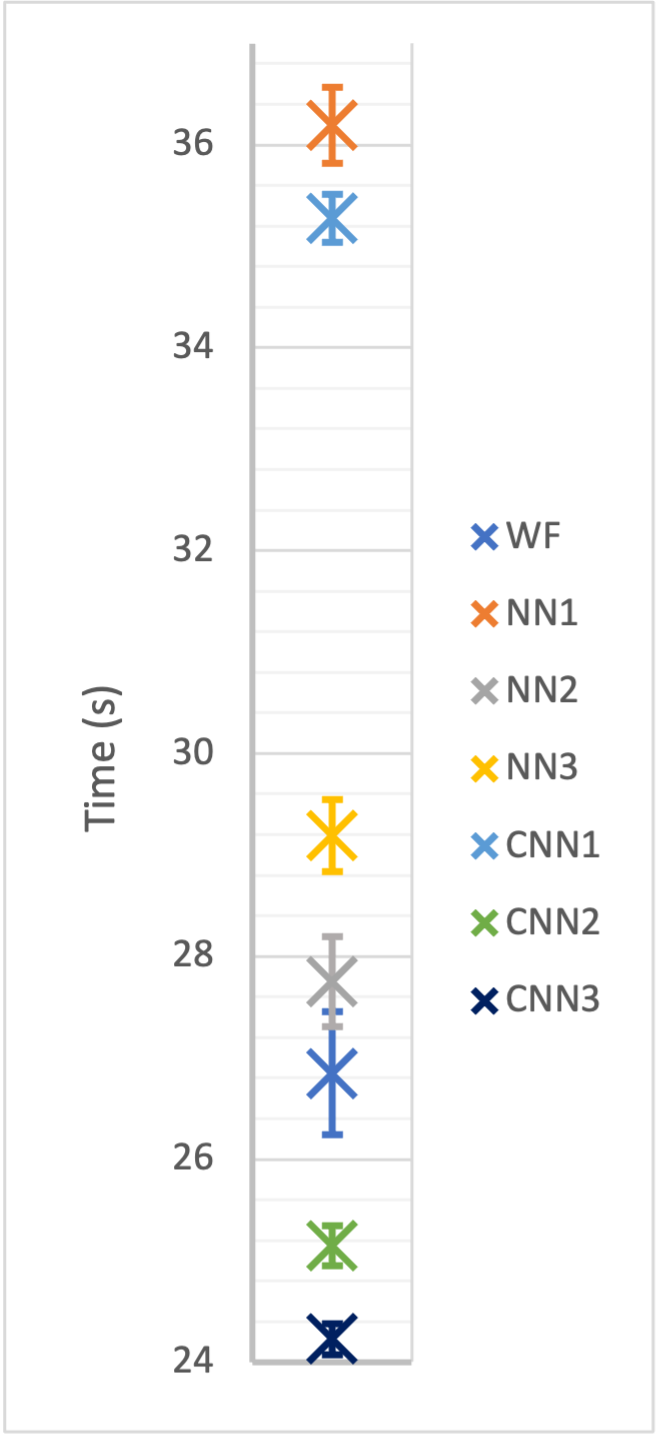
\includegraphics[width=0.65\textwidth]{Figures/H1_Time.png}
        \caption{Lap time comparison for controllers on the RedBull track (from Excel file)}
        \label{h1_time}
    \end{minipage}\hfill
    \begin{minipage}{0.45\textwidth}
        \centering
        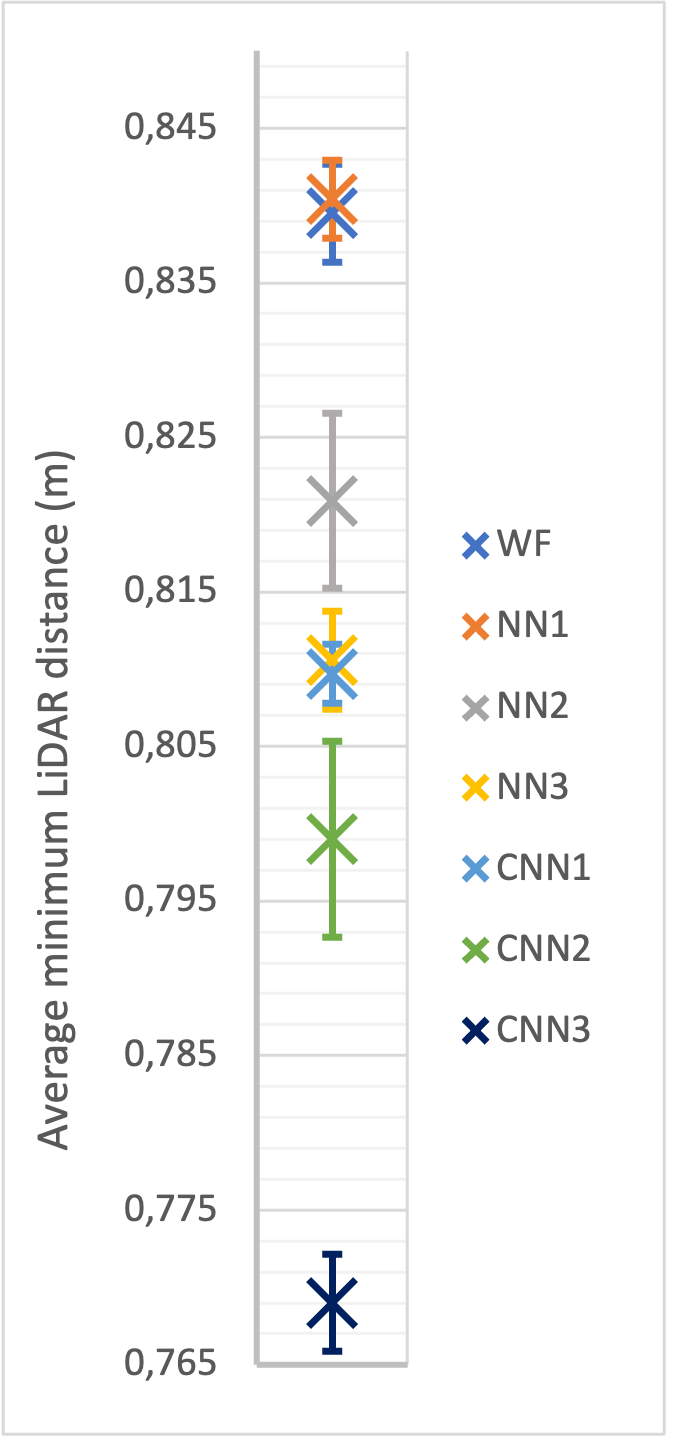
\includegraphics[width=0.65\textwidth]{Figures/H1_LiDAR.png}
        \caption{Average minimal LiDAR distance for controllers on the RedBull track (from Excel file)}
        \label{h1_lidar}
    \end{minipage}
\end{figure}

\begin{figure}
    \centering
    \begin{minipage}{0.45\textwidth}
        \centering
        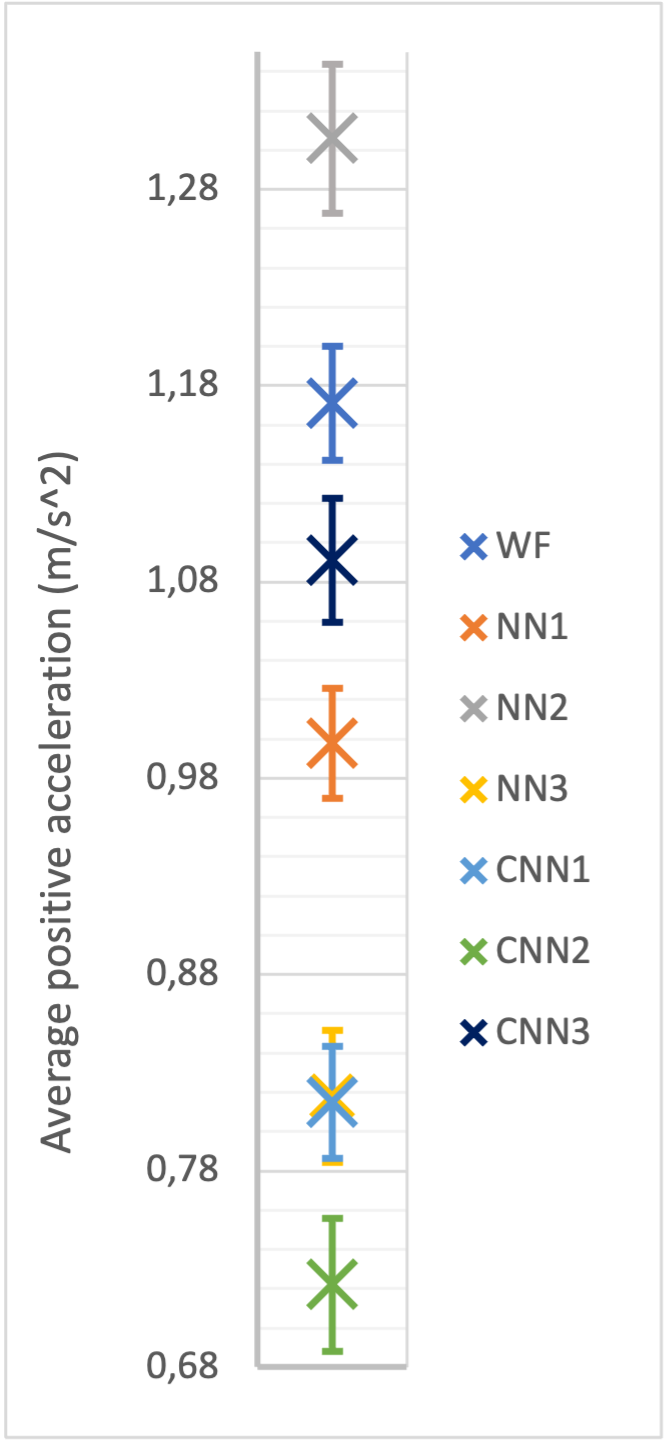
\includegraphics[width=0.65\textwidth]{Figures/H1_accel.png}
        \caption{Average acceleration comparison for controllers on the RedBull track (from Excel file)}
        \label{h1_accel}
    \end{minipage}\hfill
    \begin{minipage}{0.45\textwidth}
        \centering
        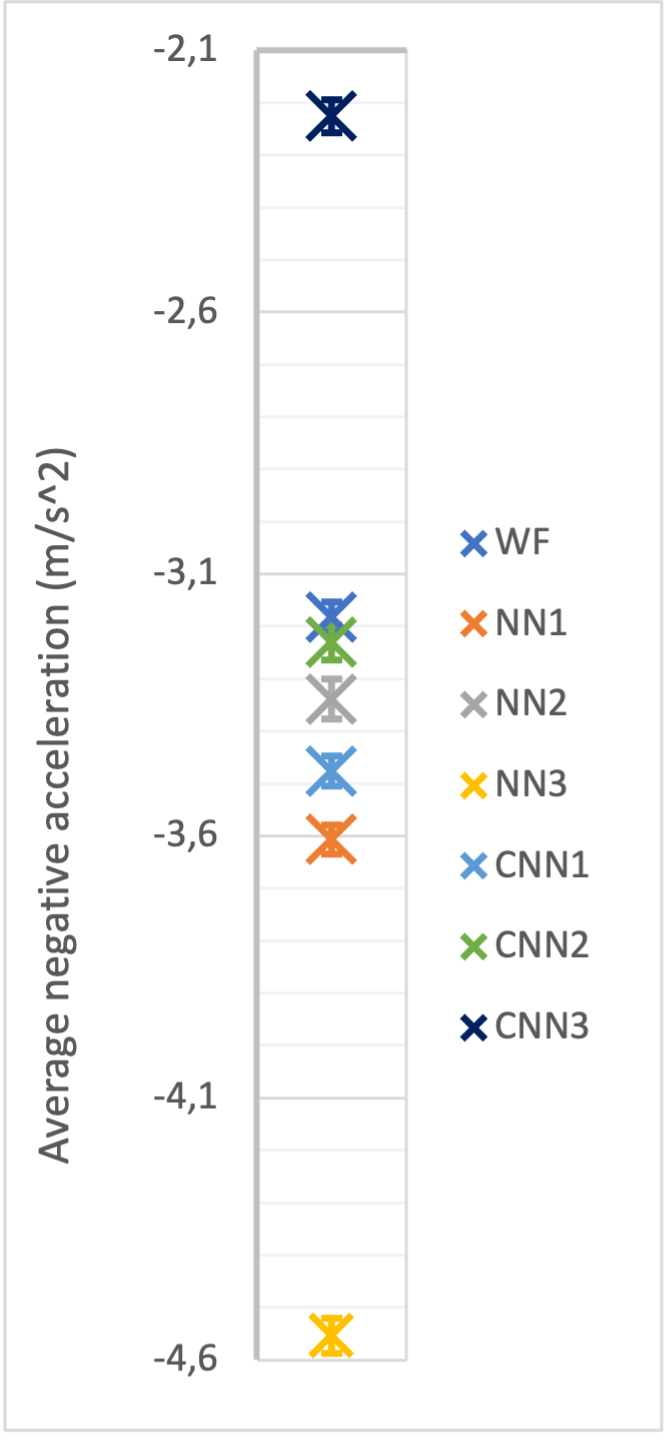
\includegraphics[width=0.65\textwidth]{Figures/H1_decel.png}
        \caption{Average deceleration comparison for controllers on the RedBull track (from Excel file)}
        \label{h1_decel}
    \end{minipage}
\end{figure}

\begin{figure}
	\centering
	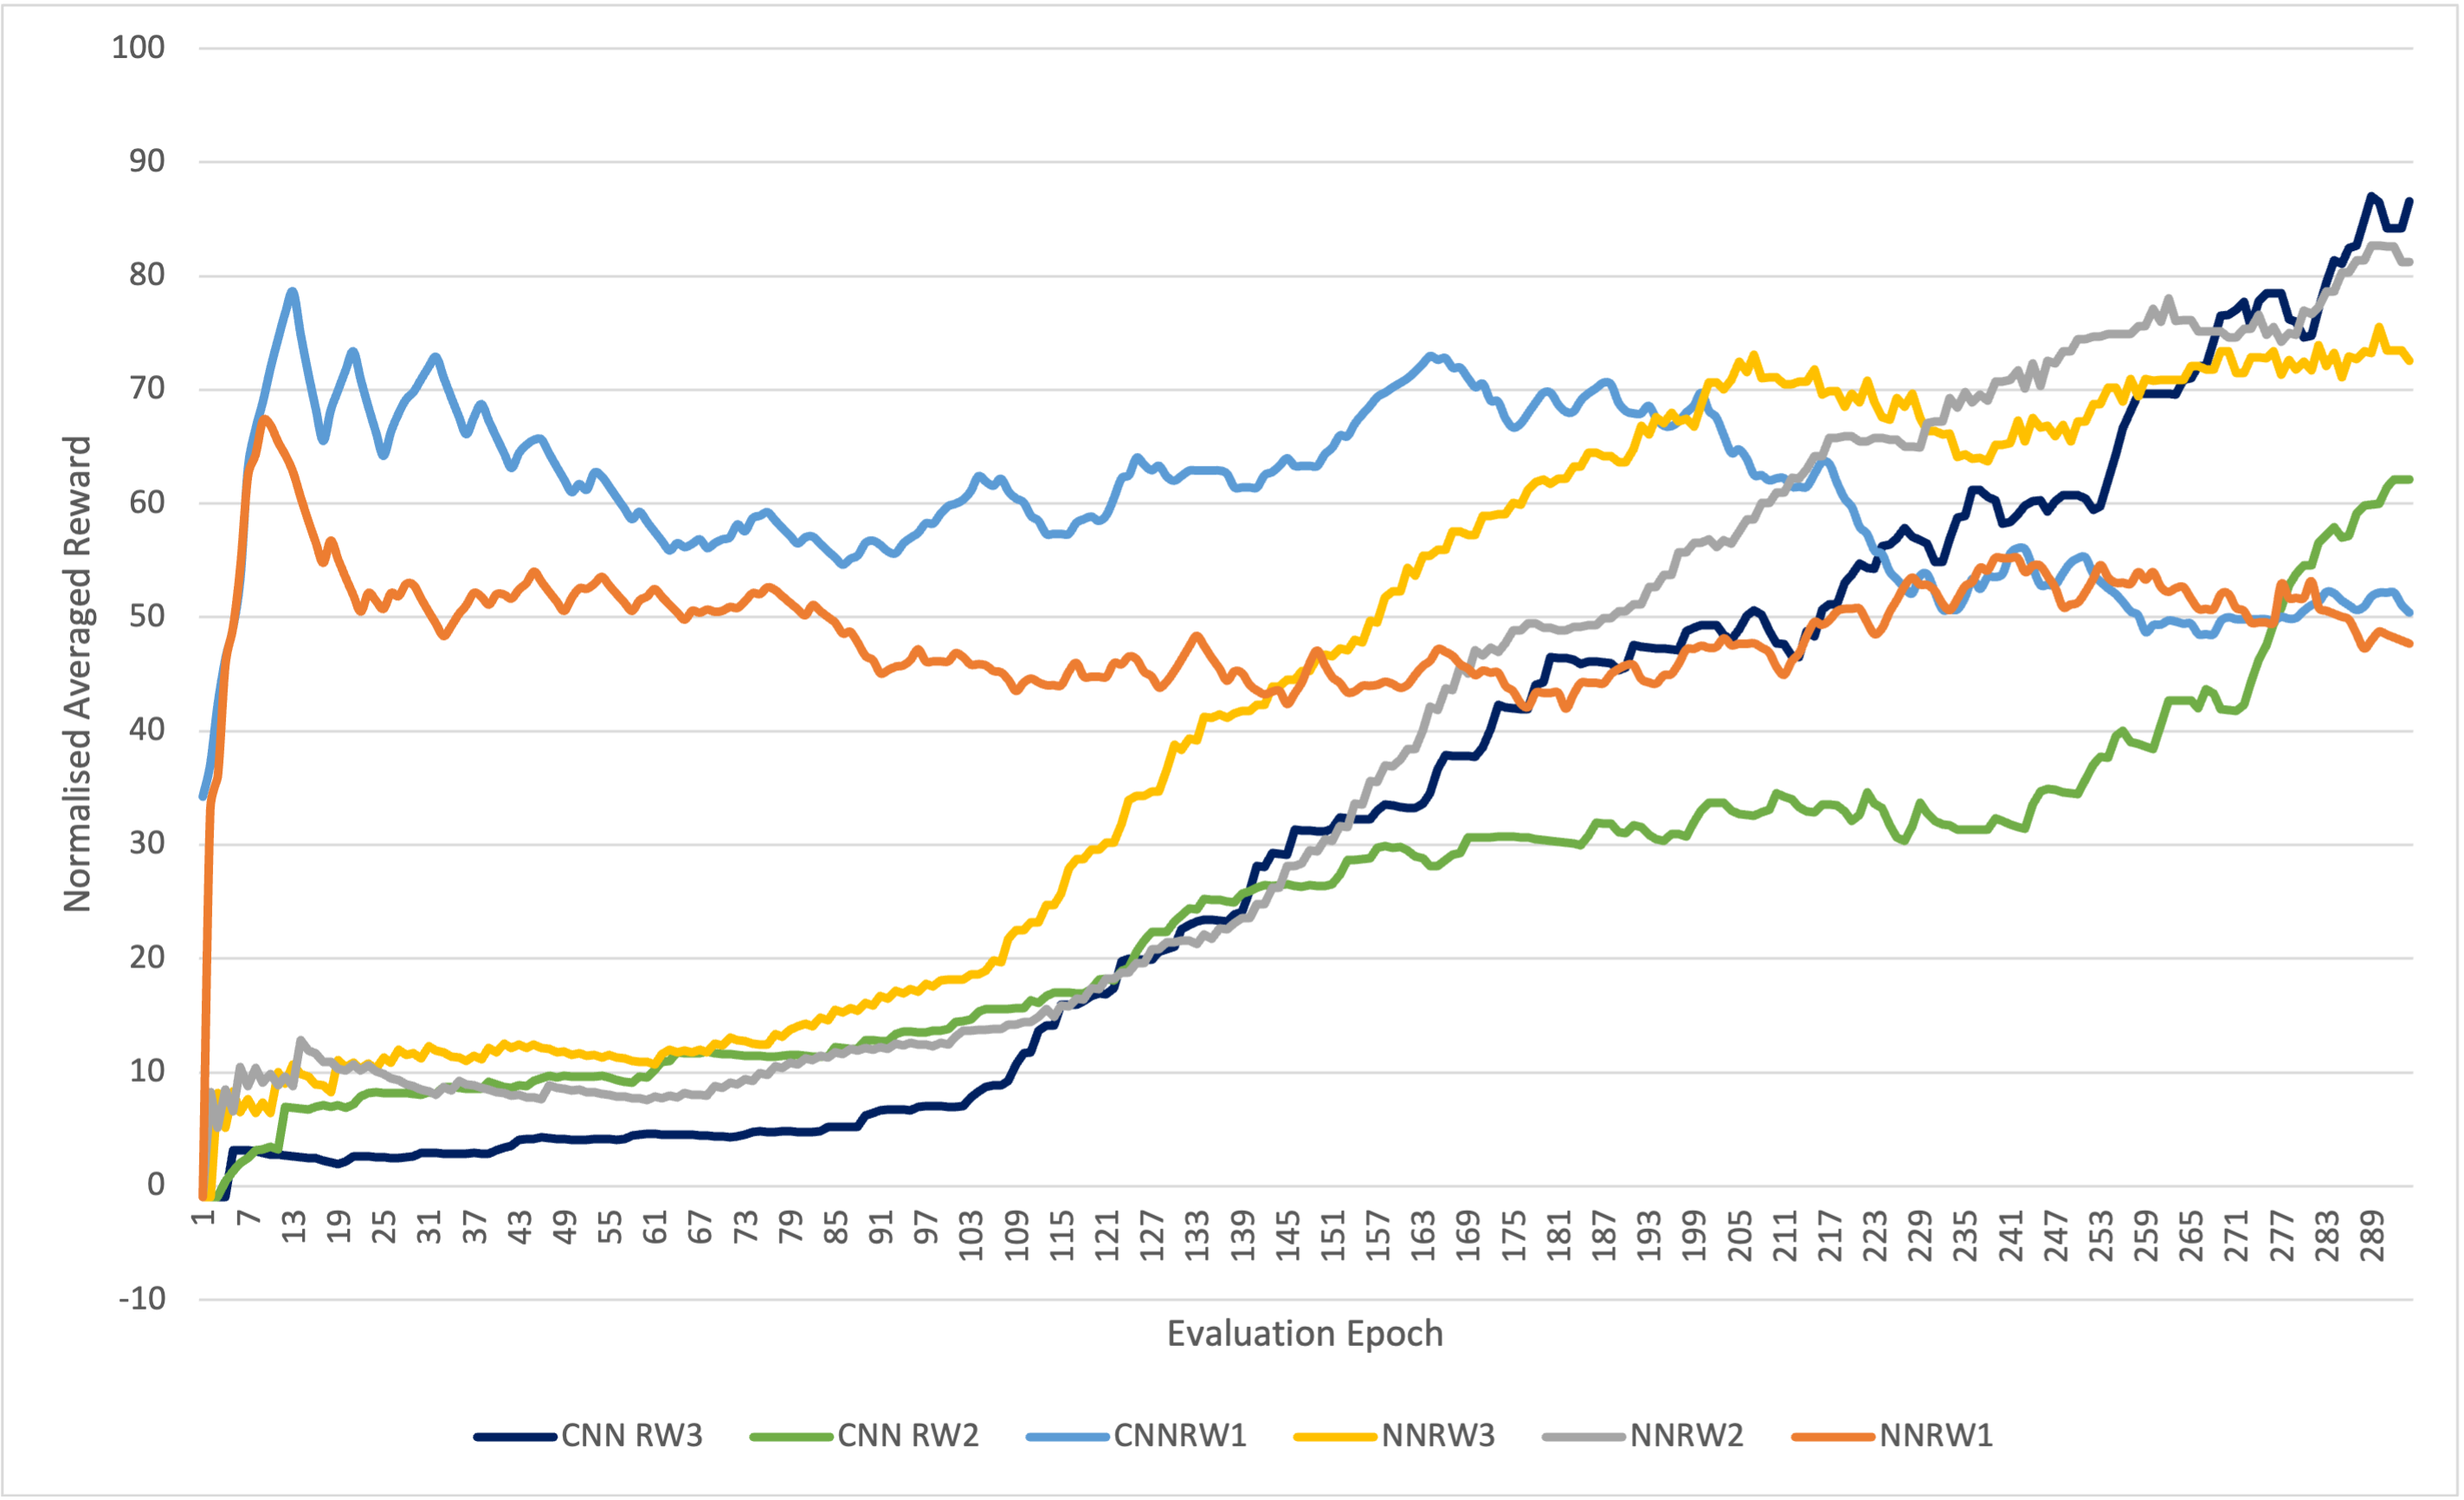
\includegraphics[scale=0.65]{Figures/eval_score.png}
	\caption{Comparison of average rewards on an evaluation epoch in function of the epoch for the different DQN controllers (from Excel file)}
	\label{comparison_eval}
\end{figure}

\subsection{Hypothesis n°2}
When looking at the comparison between the lap time, average minimal LiDAR distance and average acceleration/deceleration metrics on the RedBull track (Figures \ref{h1_time}, \ref{h1_lidar}, \ref{h1_accel} and \ref{h1_decel}), we can draw 3 conclusions regarding Hypothesis n°2 (\textit{CNNs offer better results over selected metrics than NNs for autonomous racing on the F1Tenth platform using data from a UST-10LX LiDAR.}):
\begin{itemize}
	\item Regarding the speed metric (time to complete a full lap), Hypothesis n°2 is verified: for each reward function, the CNN controller performs better than the NN controller.
	\item Regarding the safety metric (average minimum LiDAR distance), Hypothesis n°2 is also verified: for each reward function, the CNN controller performs better than the NN controller.
	\item Regarding the smoothness metric (average acceleration/deceleration), Hypothesis n°2 is verified for reward functions 1 and 2.
\end{itemize}

Hypothesis n°2 was then checked using the P-Value method, similarly to Subsection \ref{reflexions_h1}, using the following hypotheses:

\begin{itemize}
	\item \textbf{Null Hypothesis (H0)}: There is no real advantage provided by CNNs over NNs using the same reward function.
	\item \textbf{Alternative hypothesis (H1)}: There is a real advantage provided by CNNs over NNs using the same reward function.
\end{itemize}

Using the standard value of Alpha = 0.05 and an independent two-tailed T-test, the results for all metrics were found to be significant; more details are available in the Excel file at \url{https://github.com/HL-Boisvert/MSc_Project_HW}. \\
To conclude, Hypothesis n°2 is verified for all metrics and reward functions apart from reward function 3 for the smoothness metric.

\subsection{Hypothesis n°3}
Hypothesis n°3 (\textit{DRL-based controllers can generalise to new race tracks without affecting too much the metrics}) was verified by comparing on the Monaco track the performance of the CNNs trained on the RedBull track to those trained on the Monaco track. \\
The P-values were then calculated, still using the standard value of Alpha = 0.05 and an independent two-tailed T-test (Table \ref{pvalues}).

\begin{table}[H]
\centering
\begin{tabularx}{\textwidth}{||X|X|X||} 
\hline
 Metric & Reward Function 2 & Reward function 3\\ [0.5ex] 
 \hline\hline
Time ($s$) & 0.99$>$0.05 & 0.64$>$0.05\\[0.5ex] 
 \hline
Average Positive Acceleration ($m/s^2$) & 0.74$>$0.05 & 0.98$>$0.05\\[0.5ex] 
 \hline
 Average Negative Acceleration ($m/s^2$)  & 0.77$>$0.05 & 0.34$>$0.05\\[0.5ex] 
 \hline
 Average Minimal LiDAR distance ($m$) & 0.91$>$0.05 & 0.93$>$0.05\\[0.5ex] 
 \hline
\end{tabularx}
\caption{P-Values for all metrics on Monaco Track when comparing DQN controllers trained on Monaco or RedBull tracks}
\label{pvalues}
\end{table}

All P-Values are larger than 0,05, meaning there is a significant statistical difference between the controllers trained on the Monaco track and those trained on the RedBull track. \\
The metric are compared in Table \ref{h3metricscomparison} and in Figures \ref{h3_time}, \ref{h3_accel}, \ref{h3_decel}, \ref{h3_lidar}: The Monaco-trained controllers perform better on the speed metric by around 10\%, however, the RedBull trained controllers perform better on the safety metric by around 5\%. The performance is similar on the smoothness metric. \\
Furthermore, we can also see that even the CNNs trained on a different track perform better than the Wall Following controller on all metrics. \\
To conclude, Hypothesis n°3 is considered verified as there is no major difference in performance on the Monaco track for controllers trained on Monaco or a different track. Those results show that CNNs are able to generalise to new tracks without significant performance changes.

\begin{table}[H]
\centering
\begin{tabularx}{\textwidth}{||X|X|X|X|X|X|X|Xs||} 
\hline
Controller & Total Time ($s$) & Average Positive Acceleration ($m/s^2$)& Average Negative Acceleration ($m/s^2$) & Maximum Acceleration ($m/s^2$) & Maximum Deceleration ($m/s^2$) & Average Minimum LiDAR Range ($m$)\\ [0.5ex] 
 \hline\hline
CNN RW2 & +10.55\% & +3.23\% & -3.20\% & +1.16\% & -1.35\% & +2.50\% \\[0.5ex] 
 \hline
CNN RW3 & +9.95\% & +5.95\% & -3.51\% & 0.92\% & -9.29\% & +7.23\% \\[0.5ex] 
 \hline
\end{tabularx}
\caption{Comparison of metric changes on the Monaco track when going from Monaco trained controllers to RedBull trained controllers}
\label{h3metricscomparison}
\end{table}


\begin{figure}
    \centering
    \begin{minipage}{0.45\textwidth}
        \centering
        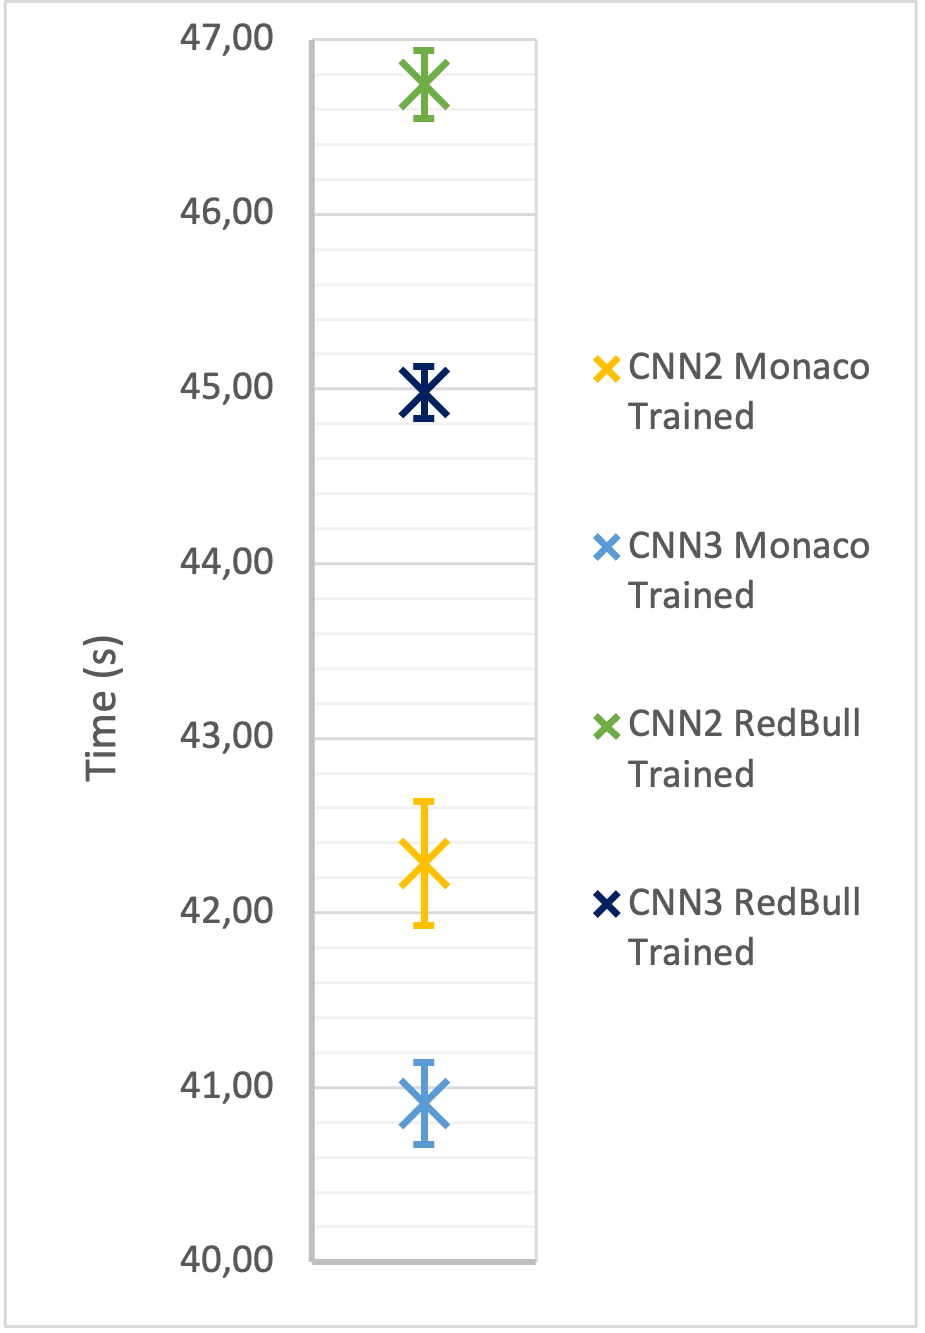
\includegraphics[width=0.8\textwidth]{Figures/H3_Time.png}
        \caption{Lap time comparison on the Monaco track (from Excel file)}
        \label{h3_time}
    \end{minipage}\hfill
    \begin{minipage}{0.45\textwidth}
        \centering
        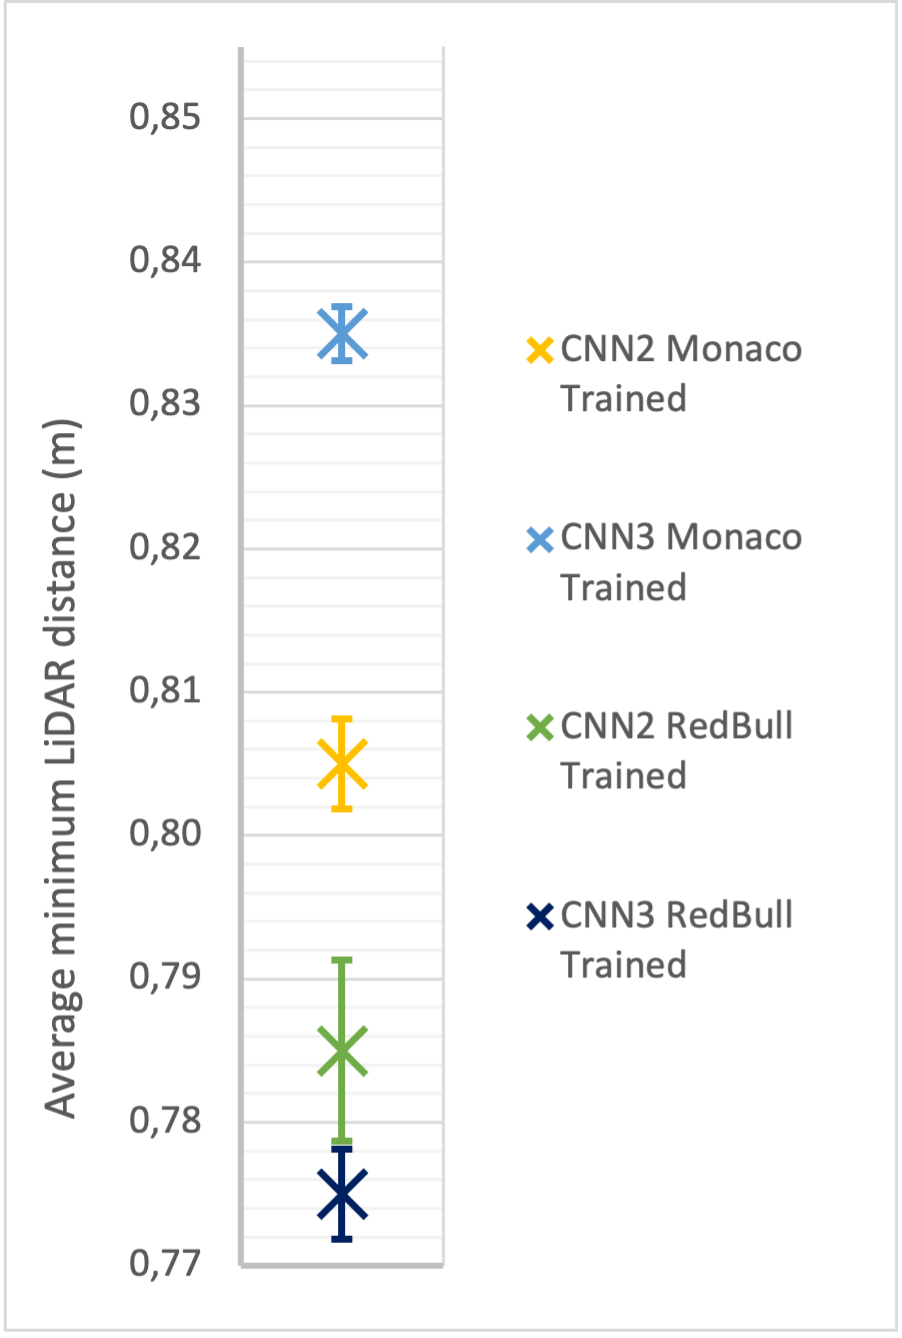
\includegraphics[width=0.8\textwidth]{Figures/H3_LiDAR.png}
        \caption{Average minimal LiDAR distance on the Monaco track (from Excel file)}
        \label{h3_lidar}
    \end{minipage}
\end{figure}

\begin{figure}
    \centering
    \begin{minipage}{0.45\textwidth}
        \centering
        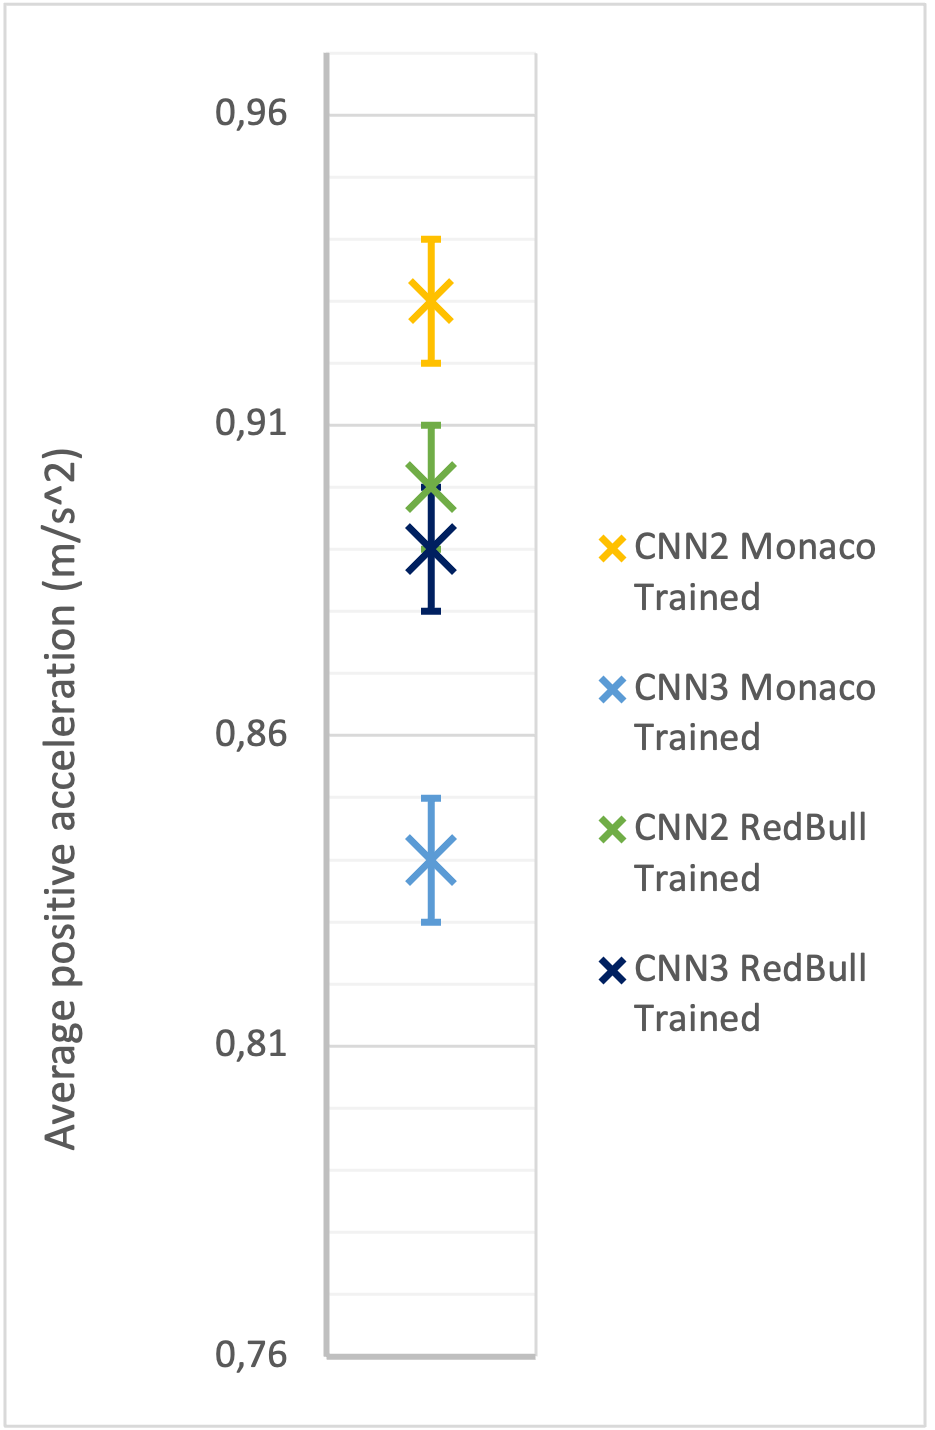
\includegraphics[width=0.8\textwidth]{Figures/H3_accel.png}
        \caption{Average acceleration comparison on the Monaco track (from Excel file)}
        \label{h3_accel}
    \end{minipage}\hfill
    \begin{minipage}{0.45\textwidth}
        \centering
        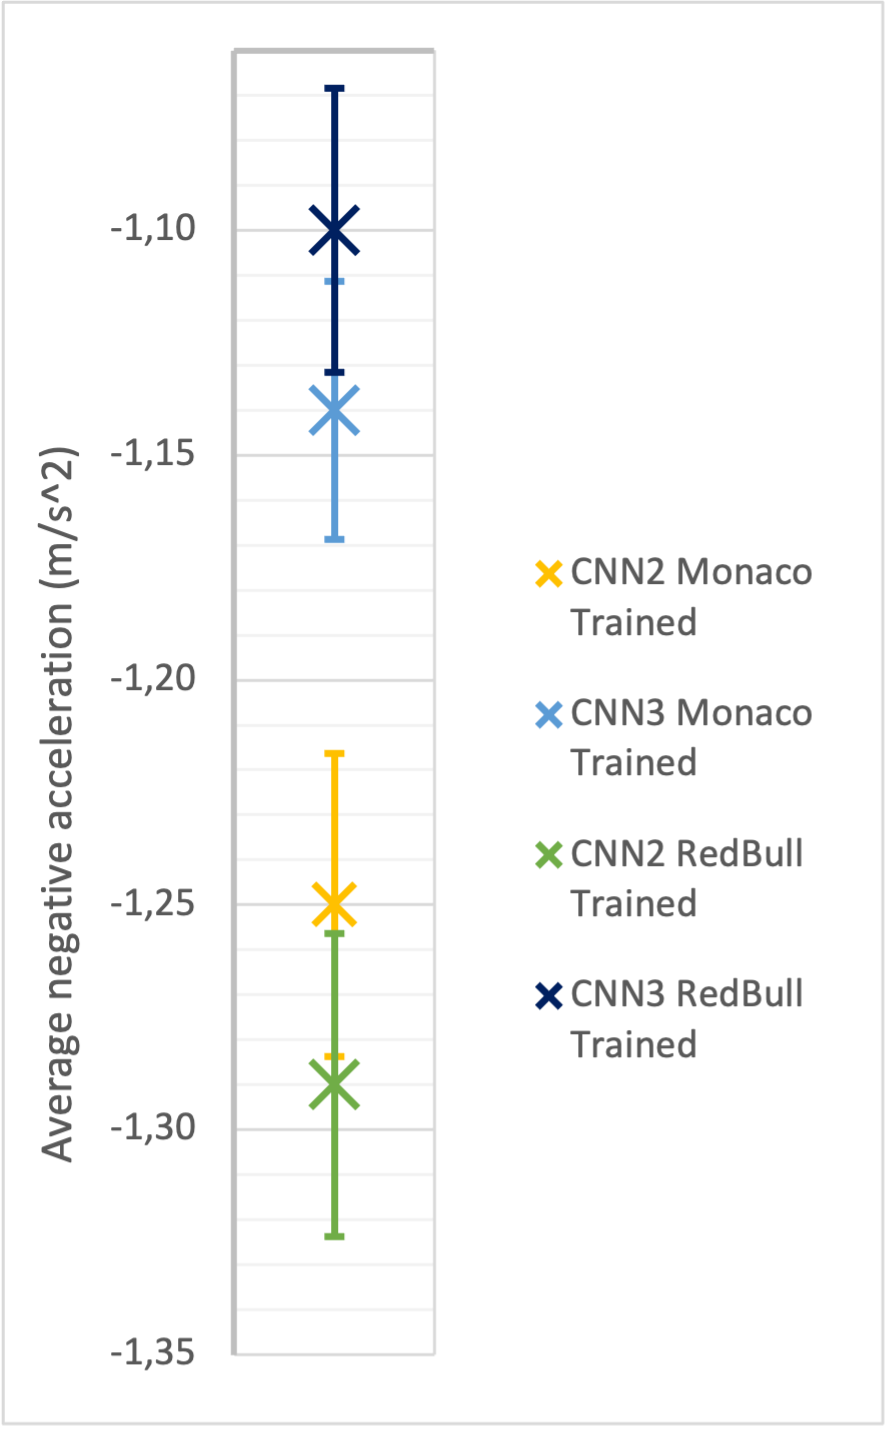
\includegraphics[width=0.8\textwidth]{Figures/H3_decel.png}
        \caption{Average deceleration comparison on the Monaco track (from Excel file)}
        \label{h3_decel}
    \end{minipage}
\end{figure}


\subsection{Hypothesis n°4}
Concerning Hypothesis n°4 (\textit{The sim2Real gap is negligible (minor changes of the metrics) and doesn't affect the performance of the controllers implemented.}), we first looked at the Wall Following controller. Once the PID was tuned, there was no significant statistical difference between the simulator and the physical car, with $p-value=0,019<0,05$ for the speed metric and $p-value=0,039<0,05$ for the safety metric. \\
Looking at the CNN with reward function n°3, there was also no significant statistical difference, with $p-value=0,046<0.05$ for the speed metric and $p-value=0,033<0.05$ for the safety metric. \\
Table \ref{h4comparisons} shows that the only significant (>5\%) difference between the simulator and the physical car is the 20\% time increase for the CNN controller using reward function n°3. \\
Compared to manual driving, we can conclude that both those controllers are performing better regarding both the speed and safety metrics, with the DQN controller performing the best. \\
To conclude, Hypothesis n°4 cannot be considered verified as there is a significant increase in the time to complete a full lap on the CNN with reward function n°3.

\begin{table}[H]
\centering
\begin{tabularx}{\textwidth}{||X|X|X||} 
\hline
 Controller & Time ($s$) & Average Minimum LiDAR range ($m$) \\ [0.5ex] 
 \hline\hline
Wall Following & +0.52\% & -2,56\% \\[0.5ex] 
 \hline
CNN RW3 & +20.39\% & -0.55\% \\[0.5ex] 
 \hline
\end{tabularx}
\caption{Comparison of metric changes when going from the simulator to the physical car}
\label{h4comparisons}
\end{table}


There are four limitations to Hypothesis n°4:
\begin{enumerate}
	\item The lack of the speed input because of the unreliable odometry, which means the metrics that depended on the speed measurement couldn't be assessed
	\item The lack of data for a complete lap of the track with the DQN controller
	\item The lack of data at speeds higher than 4m/s
	\item The lack of data for DQN controllers other than the CNN with reward function n°3
\end{enumerate}

\section{General Conclusions}
\label{generalconclusions}

We can now make some general conclusions from this project: 
\begin{itemize}
	\item DRL has proven to be quite time-consuming compared to Wall Following, especially the training; however, this is a hardware limitation, and the training process could be improved by fine-tuning the hyper-parameters.
	\item Choosing an appropriate reward function is critical: with an inappropriate function, the DQN controller cannot complete a full lap on the Monaco and Silverstone tracks.
	\item When using an appropriate reward function (n°2 and 3), DQN performs better than Wall Following on all metrics, even on never-seen-before tracks (H1).
	\item CNNs provide a real advantage over NNs according to all metrics (H2).
	\item With our parameters, DQN can generalise to new tracks (H3), although not perfectly (compared to a controller specifically trained for the track). 
	\item There is a non-negligible Sim2Real gap both for Wall Following and DQN. Regarding Wall Following, once the PID is tuned again, the controller performs similarly to the simulator. Regarding DQN, the controller had an issue preventing it from completing a full lap. However, when extrapolating, the DQN controller still performs better than Wall Following and Manual driving according to the speed and safety metrics. The Sim2Real gap is visible when comparing the performance of DQN on the physical car to the one in the simulator, especially regarding the speed metric (H4).
	\item Our results have several limitations, mainly due to time constraints, which could be an area of improvement in future works, listed in Section \ref{futureworks}.
\end{itemize}


\section{Future works}
\label{futureworks}
This dissertation introduced a well-defined protocol in Chapter \ref{Chapter6}; because this experimental protocol is quite flexible, the process could be extended to other DRL state-of-the-art methods, such as DDPG and TD3, following the same methodology. \\
A first improvement to the experimental protocol would be to fine-tune the different DQN hyper-parameters: learning rate $\alpha$, discount factor $\gamma$, greediness $epsilon$, epsilon decay, and size of the replay buffer. This would make sure that the training process is as efficient as possible. \\
A second improvement would be to train the controllers for longer to then test their limits; this couldn't be done due to hardware and time constraints. \\
A third improvement to the experimental protocol would be verifying hypothesis n°3 more rigorously. The protocol used here to verify this hypothesis was to train the DQN controller on the RedBull racetrack before testing it on the Silverstone and Monaco tracks. The underlying assumption was that those three tracks offered a comparable level of challenge, but this hasn't been proven. Because the underlying assumption may be false, it makes the assessment unreliable. A way to improve this would be by defining a metric to quantify the difficulty offered by a specific race track based on the length, minimal track width and minimum curve radius. This could be implemented using a Support Vector Machine (SVM) with the shape of the track as an input, as introduced in \cite{futurework}.\\
A fourth improvement to the experimental protocol would be to develop a more advanced simulator to perform the training, for example, by using a more accurate kinematic model rather than the Bicycle model we used.
A fifth and last improvement would be to use the car's speed as an input for the DQN controllers, which could improve the performance regarding the speed metric.